\documentclass[11pt]{book}

\usepackage{graphicx}
\usepackage[dvipsnames]{color}
\usepackage[hidelinks]{hyperref}
\usepackage[square,numbers]{natbib}
\usepackage[square,numbers]{natbib}
\bibliographystyle{abbrvnat}
%pPara poder modificar los margenes
\usepackage{vmargin}
%Para usar el español
\usepackage[spanish]{babel}
\usepackage[utf8]{inputenc}
\usepackage{hyperref}
\bibliographystyle{plain}
\usepackage{hyperref}
\begin{document}
%Portada
\setpapersize{A4}
\begin{titlepage}
	\centering
	{
\includegraphics[width=0.8\textwidth]{logo}\par}
	\vspace{1cm}
	{\Large Facultad de Ingeniería Informática \par}
	\vspace{3cm}
	{\scshape\Huge Aplicación web de soporte al Aprendizaje-Servicio \par}
	\vspace{5cm}
	{\textbf\Large Autores \par}
	{\Large Daniela-Nicoleta Boldureanu (Grado en Ingeniería del Software)\par}
	{\Large Victoria Gnatiuk Romaniuk (Grado en Ingeniería Informática)\par}
	{\Large Jesús Sánchez Granado (Grado en Ingeniería Informática)\par}
	\vspace{1cm}
	{\textbf\Large Tutores \par}
	{\Large Simon Pickin \par}
	{\Large Manuel Montenegro Montes \par}
	
\end{titlepage}

%Indice

\tableofcontents
\newpage
\listoffigures

\chapter{Tecnologías utilizadas}
A continuación, se hablará sobre las tecnologías utilizadas explicando brevemente que son y los motivos por los que han sido seleccionadas.

\section{Node.js} 
Node.js \cite{node} es un entorno de ejecución asíncrono dirigido por eventos. Funciona a base de promesas, es decir, funciones que devolverán un resultado en algún momento del futuro. Las promesas se pueden encadenar una tras otra, recibiendo cada una el resultado de la anterior.\\\\
Esta forma de conseguir concurrencia es distinta a la manera más común que es utilizando cierres de exclusión mutua o candados. Los candados funcionan de la siguiente manera: si durante la ejecución de un programa concurrente un elemento es compartido por varios hilos, el resultado dependerá de las operaciones y el orden en que se lleven a cabo las mismas en dicho elemento. Para evitar que dos hilos accedan de manera simultánea a un mismo recurso, hay que ``bloquear'' ese recurso utilizando candados, llegando a la situación conocida como exclusion mutua ,pero cuando hay varios procesos concurrentes puede darse la situación de que el proceso A esté esperando a que el proceso B libere un recurso, y al mismo tiempo B espera que A libere un recurso. Esta situación se conoce como \emph{deadlock} o interbloqueo y es un bloqueo infinito.\\\\
Node.js no utiliza cierres de exclusión mutua o candados, por lo que es imposible que el programa alcance el estado de \emph{deadlock}, lo que lo hace bastante adecuado para desarrollar sistemas escalables.\\
Otro motivo para continuar con esta tecnología es que Daniela ya tenía conocimiento previo de este entorno y es una tecnología que venía impuesta por el proyecto.

\section{Angular}
Angular \cite{angular} es un \emph{framework} para la construcción de aplicaciones de página única (SPA a partir de ahora) que utiliza HTML y Typescript. Angular sigue el patrón modelo-vista-controlador, el cual consiste en separar la aplicación en tres partes:
\begin{itemize}
	\item Modelo: Es la piedra angular del patrón, se encarga de manejar los datos y la lógica de la aplicación.
	\item Vista: Es la parte que se le muestra al usuario.
	\item Controlador: Es la parte que se encarga de comunicar a la vista y al modelo. El controlador recibe los eventos de interacción del usuario a través de la vista y se los pasa al modelo, el cual hace las operaciones necesarias y devuelve los resultados al controlador, quien se los pasa a la vista para mostrárselos al usuario.
\end{itemize}


El uso de Angular venía impuesto por el trabajo realizado con anterioridad y, aunque es una tecnología con la que ningún miembro del equipo estaba familiarizado, es cierto que el diseño de aplicación de página única hace mucho más liviana la ejecución de la aplicación por parte del usuario, al no tener unos tiempos de espera tan grandes como los que tendría al cargar de nuevo cada página. Esto hace de Angular una buena elección para un trabajo de esta índole.

\section{GitKraken}
Gitkraken es un cliente de Git con interfaz de usuario la cual se puede conectar a distintas plataformas de Git, haciendo de intermediario entre el usuario y el repositorio de Git, el cual en este caso está alojado en Github. Hemos escogido esta interfaz para nuestro control de versiones porque permite trabajar desde Windows sin necesidad de conocer los comandos de Git. A diferencia de otros clientes de Git, tiene una representación gráfica muy intuitiva que permite ver la distribución de las ramas, los \emph{commits} y su evolución, como se puede observar en la Figura \ref{Figura 1}, y además permite resolver los conflictos generados al mezclar las distintas ramas de desarrollo dentro de la propia aplicación de una manera bastante sencilla. Esto, sumado a la experiencia previa de Victoria con la aplicación, ha hecho que sea seleccionada como herramienta de control de versiones.
\begin{figure}
	\centering
	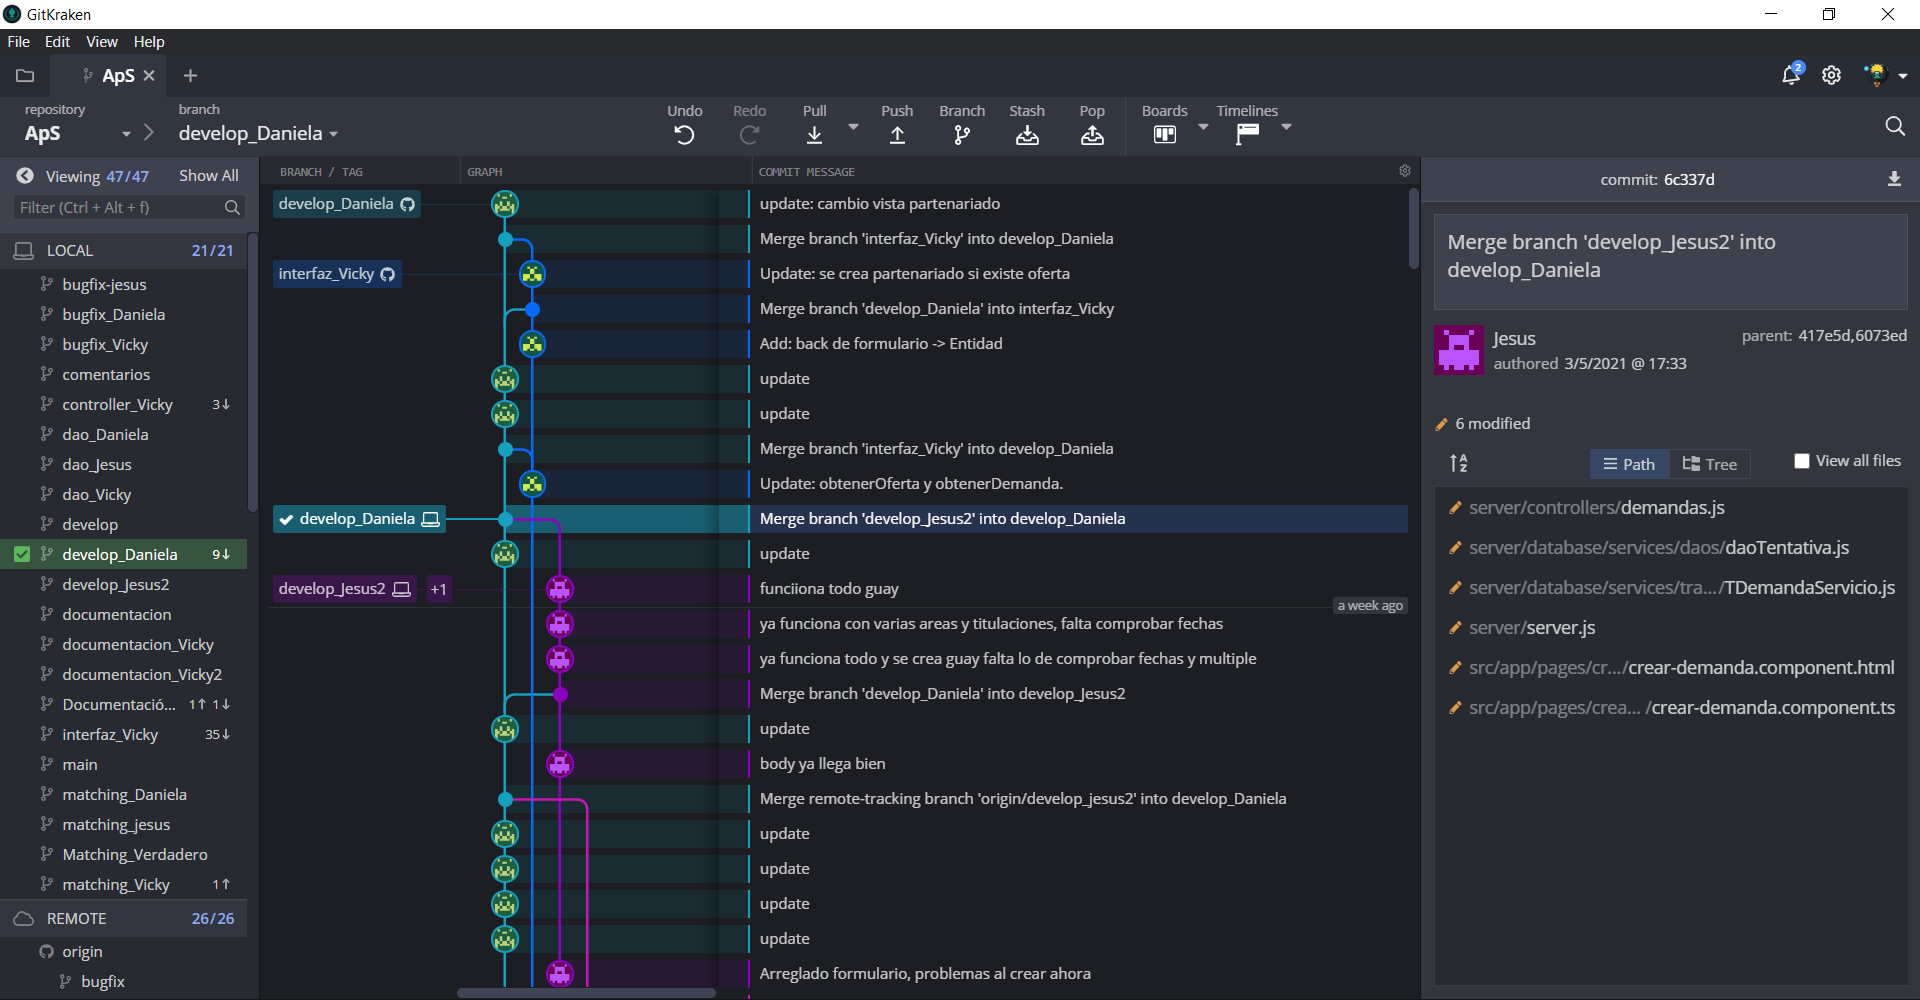
\includegraphics[scale=0.4]{gitkraken}
	\caption{GitKraken: Información de una rama de desarrollo}
	\label{Figura 1}
\end{figure}

\section{Pivotal tracker}
Pivotal tracker es una herramienta de \emph{product planning} y administración de tareas diseñada para equipos de desarrollo que siguen metodologías de diseño ágiles.
Esta herramienta permite crear historias de usuario y asignarles una puntuación del 1 al 5 indicando su dificultad y/o tiempo invertido en dichas tareas. Además, permite cambiar el estado de las tareas (empezado, finalizado, en revisión, etc.) y cualquier cambio en el estado de dichas tareas se informa por correo de manera automática a quien esté involucrado en ella.
También permite ver las tareas completadas y rechazadas y generar gráficos indicando el esfuerzo realizado, como el que podemos ver en la figura \ref{Figura 2}. Esta tecnología fue sugerida por Victoria y nos ha facilitado mucho tanto la organización como el seguimiento de nuestros avances.

\begin{figure}
	\centering
	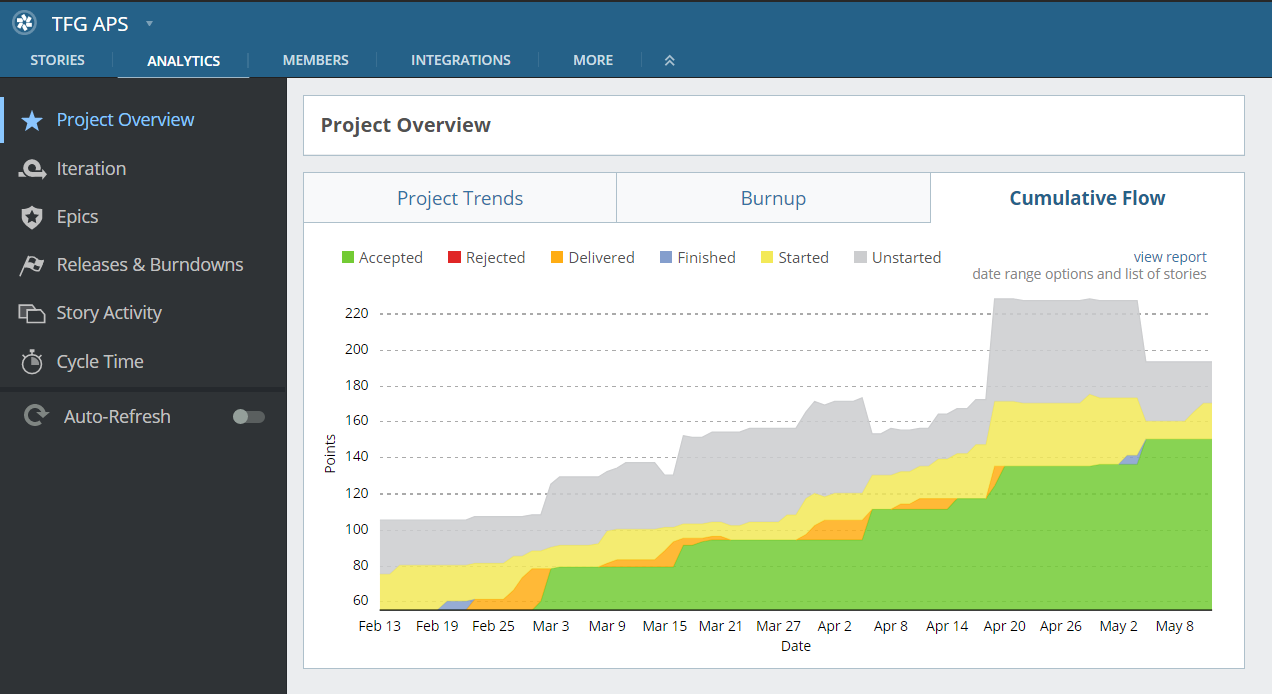
\includegraphics[scale=0.6]{pivotal}
	\caption{Pivotal tracker: Estadísticas de historias}
	\label{Figura 2}
\end{figure}

\section{\LaTeX}
\LaTeX es un lenguaje de creación de documentos escritos utilizado comúnmente en el mundo académico, que es una de las principales razones por la que lo hemos escogido para redactar nuestra memoria, a pesar de que ningún integrante del grupo tuviera experiencia previa con ello. A diferencia de otros procesadores de texto, como Microsoft Word o LibreOffice Writer, se escribe el texto plano y se formatea dicho texto con etiquetas. 

\section{MySQL}
Aunque nuestro proyecto continúa el trabajo realizado por David Jiménez del Rey, el cual ya contaba con un sistema gestor de bases de datos, dicho sistema era MongoDB. Como los datos que se iban a manejar en la aplicación eran en su mayoría relacionales se tomó la decisión de utilizar MySQL para la base de datos. Dado que todos los componentes del grupo tenían experiencia previa en bases de datos SQL fue un cambio bien recibido.

\section{Modelio}	
Modelio es un entorno de modelado \emph{open-source} el cual permite trabajar con un amplio rango de modelos y diagramas. Dado que ya se contaba con experiencia previa en esta herramienta por parte de todos los miembros del equipo, se ha escogido para realizar los modelos de datos necesarios para la aplicación.

\section{MySQL Workbench}
MySQL Workbench es una herramienta para diseño, desarrollo y administración de bases de datos relacionales. 
Cuenta con funcionalidades de validación de esquemas y modelos y promueve las mejores prácticas de los estándares de modelado de datos. También promueve los estándares de diseño específicos de MySQL para evitar errores al generar esquemas relacionales o creando bases de datos MySQL. Por estos motivos, junto con su relativa simplicidad, es por lo que se ha elegido esta herramienta para hacer los diagramas de entidad-relación.

\chapter{Contribución}
	\section{Victoria Gnatiuk Romaniuk}
	La primera fase era una fase de investigación así que en esta fase todos hemos investigado y no hay ninguna tarea individual que destacar.\\\\
	En la segunda fase del proyecto Victoria se ha encargado de arreglar algunos \textit{bugs} del trabajo anterior. Los \textit{bugs} eran fáciles de arreglar, uno de ellos era que en el formulario de registro en los campos correo, nombre y apellidos se pedía al usuario que introdujera lo mismo, que era el nombre. Otra cosa que no \textit{bug}, era que al editar el perfil de usuario se pedía volver a aceptar las condiciones de uso, cosa que veíamos innecesaria.\\\\
	En la tercera fase del TFG Victoria se ha encargado de continuar el modelo de dominio y el modelo de datos usando Modelio. En paralelo ha creado las tablas \textbf{profesor\_externo, iniciativa, anuncio\_servicio, demanda\_servicio, oferta\_servicio, partenariado, proyecto, colaboracion, newsletter y entidad\_demanda} en la base de datos. También ha creado las tablas que alojan los valores de los enumerados como la tabla \textbf{area\_implemetación, necesidad\_social, area\_conocimiento, universidad, titulacion\_local} y las tablas intermedias que permiten conectar las tablas de los enumerados con las tablas que las referencian. Con crear las tablas nos referimos a crear la estructura, definiendo los nombres de los campos y los tipos de datos, y creando restricciones entre las tablas.\\
	Una vez todas las tablas fueron creadas usando MySql Workbench 8.0 CE, Victoria creó el modelo relacional a partir del fichero SQL. Después hubo que distribuir todas las tablas en los cuatro grupos explicados en el capítulo \ref{fig:relacional} para que todas las tablas fueran debidamente visibles.\\\\
	En la fase cuatro Victoria se ha encargado de desarrollar el DAO llamado \textit{Tentativa} que implementa el acceso a la base de datos del grupo de tablas llamado \textit{Anuncios de servicio} que se puede ver en la Figura \ref{fig:anuncios}. La creación de este DAO ha supuesto la necesidad de la creación de tres \textit{transfers} que alojan los datos del elemento Anuncio de servicio, Demanda de servicio y Oferta de servicio. Los daos han sido implementados usando Knex.js, una librería que facilita las consultas a la base de datos. En el DAO \textit{Tentativa} se crearon las funciones CRUD, 3 de cada tipo concretamente. Dos de ellas eran las de la oferta y la demanda y la tercera, la cual siempre se llama desde las otras dos, es la del anuncio de servicio. También se creo el método para obtener todas las iniciativas, todas las demandas y todas las ofertas. Además de estos métodos, se han creado otros necesarios para la creación de los formularios de crear oferta y demanda. \\
	Después de finalizar la implementación del DAO \textit{Tentativa} Victoria desarrolló en los métodos CRUD del elemento \textit{Partenariado} perteneciente al DAO \textit{Colaboración}. Este DAO implementa las tablas pertenecientes al grupo \textit{Colaboración} que se puede ver en esta Figura \ref{fig:colaboracion}.
	Después Victoria implementó en el DAO \textit{Usuarios} dos métodos para obtener cualquier tipo de usuario con el id y con el correo del usuario. Estos métodos eran necesarios para la adaptación de la página de registro y \textit{login} al nuevo sistema. Junto con Jesús, Victoria adaptó el \textit{login} al nuevo sistema.\\\\
	En la fase cinco Victoria se ha encargado de crear el método que determina la similitud que tiene los campos \textbf{area\_implementación}, perteneciente a la \textit{Oferta de servicio} y \textbf{area\_conocimiento}, perteneciente a la \textit{Demanda de servicio}. Para esto se ha tenido que crear un Excel donde los valores de los enumerados de \textbf{area\_implementación} se han colocado en la primera fila y los valores de los enumerados de  \textbf{area\_conocimiento} se han colocado en la primera columna. Posteriormente se han colocado \textit{X} para marcar la similitud entre los valores, está similitud ha sido determinada por Victoria. Después de crear el Excel se ha creado un \textit{script} con Python que leía este Excel e insertaba los emparejamientos en una tabla de la base de datos, de la cual se leerá posteriormente para determinar si estos dos enumerados pueden ser emparejados. A continuación, se creó el método que compraba estos enumerados. Se hizo este mismo proceso para determinar el emparejamiento entre \textbf{area\_implementación}, perteneciente a la \textit{Oferta de servicio} y \textbf{titulacion\_local}, perteneciente a la \textit{Demanda de servicio}.\\
	Además de estos métodos para determinar el \textit{matching}, Victoria implemento otros dos. Uno de ellos determinaba si las dos \textbf{areas\_implementación}, pertenecientes a Oferta de servicio y Demanda de servicio coinciden. El segundo método determinaba si coincidían las titulaciones de la \textit{Demanda de servicio} y las titulaciones que imparte el profesor que ha creado la \textit{Oferta de servicio}.\\\\
	En la fase cinco Victoria se ha encargado de implementar el formulario para crear la oferta de servicio y también ha desarrollado la parte \textit{back-end} del formulario para crear el partenariado por parte del profesor y por parte del socio comunitario.
	Conjuntamente con todo esto Victoria ha ido actualizando los modelos de dominio y de datos a medida que iban sufriendo cambios a causa de los cambios sugeridos por los directores del TFG. También ha mantenido actualizado el diagrama relacional a medida que la base de datos iba sufriendo cambios.
\newpage
	\section{Jesús Sánchez Granado}
La primera fase del proyecto era principalmente una fase de investigación, así que en esta fase todos hemos leído la memoria de David Jimenez del Rey y se ha aprovechado para preparar el entorno de trabajo y crear el repositorio de Github al cual se irán subiendo los avances en el proyecto. Además, de manera conjunta se realizaron pruebas de robustez en la aplicación web con el objetivo de intentar encontrar \emph{bugs} o posibles mejoras.\\\\
En la segunda fase del proyecto Jesús ha arreglado algunos \emph{bugs}. Uno de ellos era un mal redireccionamiento de un enlace y otro, más que un \emph{bug} era una mejora, pues al editar una iniciativa siempre pedía aceptar los términos y condiciones, cosa que se consideró innecesaria.\\
Algunos de estos \emph{bugs} se han dejado por hacer pues al tener que realizar cambios en la interfaz, los \emph{bugs} ya serían arreglados al reimplementar las vistas pertinentes.\\\\
En la tercera fase del proyecto, Jesús se ha encargado de crear la estructura de las tablas \textbf{profesorinterno\_oferta, estudiante\_iniciativa, estudiante\_proyecto, upload, upload-anuncioservicio, mail, uploads-colaboracion, mensaje, mensaje-anuncioservicio y mensaje-colaboracion}. En dicha estructura quedaban especificados los nombres y tipos de sus campos, sus restricciones, las claves foráneas y quedaban definidas también sus relaciones, siempre y cuando fueran con tablas de este grupo ya nombrado.\\
Una vez se crearon las tablas restantes y se unificó el formato de las mismas, Jesús realizó las conexiones entre las tablas que aun no habían sido relacionadas. Esto se debe a que para repartir la creación de tablas, estas se dividieron en grupos, y había algunas que se relacionaban con tablas de otros grupos, por lo que no se podían relacionar hasta tener la base de datos completa.\\\\
En la cuarta fase del proyecto Jesús se ha encargado de desarollar el DAO llamado \texttt{Comunicacion}, el cual implementa el acceso a la base de datos para el grupo de tablas que se puede ver en la Figura \ref{fig:comunicacion}. Para poder crear este DAO, antes ha necesitado crear los \emph{transfer} \texttt{TUpload, TMensajes, TMail} y \texttt{TNewsletter}. Estos \emph{transfer} se encargan, respectivamente, de almacenar los datos de los elementos upload, mensaje, mail y newsletter además de permitir modificarlos. Este DAO contiene las funciones CRUD, es decir, las necesarias para crear, leer, actualizar y eliminar elementos en las respectivas tablas de la base de datos, en total unas 22 funciones. \\
Esto se debe a que tanto los mensajes como los \emph{uploads} pueden pertenecer o a una colaboración o a un anuncio de servicio, por lo que cada uno tiene dos funciones distintas para su creación, una para cada caso. Además se han hecho también funciones para obtener todos los mensajes y todos los \emph{uploads} de una determinada colaboración o de un determinado anuncio de servicio.\\
Terminado el DAO en cuestión, Jesús creó los \emph{transfers} \texttt{TColaboracion, TProyecto} y \texttt{TPartenariado}, los cuales eran necesarios para la creación del DAO \texttt{Colaboracion}. Además, en dicho DAO hizo las funciones CRUD del \emph{transfer} \texttt{TColaboracion}. Tras esto, junto con Victoria, ambos adaptaron la funcionalidad de login al sistema actual.\\\\
En la quinta fase del proyecto Jesús ha creado el método que se encarga de comprobar si el periodo de disponibilidad de la demanda coincidía con el cuatrimestre o cuatrimestres especificados por el profesor en la oferta de servicio. También se cubrieron los casos en los que se consideraba que habia un ``\emph{antimatching}'', situaciones en las que aunque otros atributos coincidieran, el match no se llevaría a cabo. Por ejemplo si los periodos elegidos para la definicion del proyecto escogidos por el profesor y por el socio comunitario no fueran compatibles, aunque todos los demás atributos lo fueran, no habría \emph{match}.\\
Tras esto, y una vez Daniela y Victoria terminaron sus respectivos métodos, Jesús hizo la función ``maestra'' que agrupaba todos los métodos de \emph{matching} hechos anteriormente, después de moodificarlos ligeramente para que fuera más fácil hacer los cálculos de los resultados, teniendo en cuenta los respectivos pesos de los atributos. Una vez se ha calculado el porcentaje de \emph{matching}, si este es mayor que el 50\%, se guarda el resultado en la base de datos con el fín de notificar a los usuarios pertinentes.\\
Esta función además permite configurar los pesos de los atributos para así hacerla más versatil a la hora de priorizar qué están buscando los usuarios, de momento esto se ha hecho creando un fichero llamado \texttt{configuracion.txt} para que la función lea los valores en él descritos y los asigne.\\\\
En la sexta fase del proyecto Jesús ha implementado el formulario para la creación de una demanda de servicio. Esto, además de la creación de un fichero crear-demanda.component.html y un fichero crear-demanda.component.scss para mostrar la vista al usuario  y de un fichero crear-demanda.component.spec.ts
 y un fichero crear-demanda.component.ts para encargarse de la lógica asociada al formulario, ha supuesto además cambios en los \emph{controllers} y en el fichero de rutas. Además de esto, ha cambiado algunos campos en los formularios para hacerlos más legibles para el usuario.

\chapter{DAO}\label{cap:daos}

Tras cambiar la base de datos de MongoDB por una relacional, también era necesario reimplementar la lógica de accesos a la base de datos, por lo que se crearon cuatro \emph{Data Access Object} (DAO a partir de ahora) que se encargarían de las operaciones de cada una de las cuatro áreas definidas en el modelo de entidad-relación.

El DAO es un patrón de diseño el trata de proporcionar una interfaz para la comunicación con una base de datos u otro sistema de persistencia de datos. Esta interfaz se encarga de llevar a cabo las operaciones CRUD, es decir creación, lectura, actualización y eliminación de datos y además asegura la independencia entre la lógica de la aplicación y la capa de negocio.

Aunque no eran estrictamente necesarios dado que en javascript no hace falta declarar el tipo de los objetos, se decidió crear objetos \emph{transfer} para así tener más documentados los campos de cada tipo de objeto.
Un \emph{transfer} o \emph{Data Transfer Object} es un objeto cuya única función es guardar la información de cierto objeto y permitir su acceso y manipulación.
De esta forma, si hay algún problema, este se detectará cuanto antes y evitará que la aplicación falle repentinamente en fases más avanzadas de la ejecución.

Los objetos \emph{transfer} contienen simplemente los atributos deseados de cada tipo de objeto además de las funciones \emph{get} y \emph{set} para poder acceder y actualizar la información de dichos atributos.
En conjunto con los DAO, los \emph{transfer} ayudan aún más a la separación de capas de negocio y lógica.

Los cuatro DAO que se crearon a partir del diagrama entidad-relación son:

\begin{itemize}
	\item \texttt{DAOColaboracion}: Se encarga de manejar toda la información relacionada con los proyectos y los partenariados, desde sus participantes, ya sean profesores o estudiantes hasta los mensajes y archivos asociados a estos proyectos o partenariados. Este DAO se llama así porque tiene como piedra angular la clase \texttt{Colaboración}.
	Esta clase fue creada para hacer de padre de las clases \texttt{Partenariado} y \texttt{Proyecto} y así evitar la repetición de métodos y atributos similares. Utiliza los \emph{transfer} \texttt{TColaboracion}, \texttt{TPartenariado} y \texttt{TProyecto}.

	\item \texttt{DAOComunicacion}: Se encarga de manejar toda la información relacionada con todas las formas de comunicación disponibles, desde los mensajes y los \emph{uploads} que se pueden intercambiar durante las distintas fases de un partenariado o proyecto hasta los \emph{emails} o las \emph{newsletter} a las que se pueden suscribir los usuarios. Por lo tanto utiliza los \emph{transfer} \texttt{TUpload}, \texttt{TMensajes}, \texttt{TMail} y \texttt{TNewsletter}

	\item \texttt{DAOTentativa}: Se encarga de manejar toda la información relacionada con ofertas y demandas y sus relaciones con la titulación local ofrecida por la universidad, las áreas de servicio y las necesidades sociales que pudiera tener la demanda. 
	Al igual que antes, se creó una clase padre llamada \texttt{Anuncio} para evitar la repetición de atributos en las clases \texttt{Oferta} y \texttt{Demanda} y en sus derivadas. Este DAO también se encarga de las iniciativas, que son propuestas de proyecto realizadas por un estudiante a la espera de que se le dé el visto bueno, y de los mensajes y \emph{uploads} que pudieran tener tanto la oferta como la demanda. Para poder llevar a cabo esta función, este DAO utiliza los \emph{transfer} \texttt{TIniciativa}, \texttt{TOfertaServicio}, \texttt{TAnuncioServicio} y \texttt{TDemandaServicio}.

	\item \texttt{DAOUsuario}: Se encarga de manejar los datos pertenecientes a las distintas clases de usuario, que son: profesor interno, profesor externo, estudiante interno, estudiante externo, \emph{admin}, socio comunitario y oficina ApS.
	Además de estas clases, también interactúa con los respectivos padres de cada una de ellas y con las titulaciones locales, áreas de conocimiento y universidades que son necesarias para completar los atributos de los profesores.
	Para ello utiliza los \emph{transfer} \texttt{TAdmin}, \texttt{TEntidad} (que deberá cambiarse en un futuro por \texttt{TSocioComunitario}), \texttt{TUsuario}, \texttt{TProfesor}, \texttt{TOficinaAPS}, \texttt{TEstudiante}, \texttt{TProfesorExterno}, \texttt{TProfesorInterno}, \texttt{TEstudianteInterno} y \texttt{TEstudianteExterno}.

	
	\end{itemize}
	Se ha intentado que los DAO tengan todas las funcionalidades necesarias para que la aplicación pudiera seguir funcionando tras sufrir cambios sin necesidad de actualizar los DAO con frecuencia, pero resulta imposible saber qué nuevas funcionalidades puede adquirir la aplicación o qué cambios podría sufrir el modelo de datos así que, aunque cuenta con bastantes funcionalidades, será necesario actualizarlo sobre la marcha si en un futuro la aplicación sufre cambios.

\chapter{Conclusiones y trabajo futuro}
\section{Introducción}
En esta última sección se hablará sobre el estado actual del proyecto y sus objetivos, así como de las mejoras que se podrían realizar sobre el mismo en un futuro.\\\\

Dado que este TFG es una continuación del proyecto de David Jiménez del Rey, se comenzará exponiendo las principales diferencias del proyecto actual con este último.
\begin{itemize}
	\item La base de datos: Además de haber cambiado la base de datos de MongoDB a una base relacional, se han realizado varios cambios en el modelo 		como queda explicado en la sección 5.
	\item La capa de acceso a datos: Siguiendo el cambio en la base de datos, se han creado DTO y DAO para llevar a cabo la lógica de accesos a la BD 			como queda explicado en la sección 6.
	\item Implantación de un sistema de \emph{matching}: El proyecto del año pasado trataba las ofertas y las demandas como simétricas, es decir, teniendo los mismos atributos, pero esto no 	es así, por lo que se ha diseñado un sistema de matching como queda explicado en la sección 7.
	\item Cambios en los formularios: Debido a los cambios registrados en el modelo de datos, ha sido necesario crear algunos formularios o adaptar otros ya existentes. Esto queda mejor explicado en la sección 8.
\end{itemize}

\section{Objetivos cumplidos}
A continuación se repasarán los objetivos de este trabajo y su completitud:
\begin{itemize}
	\item \emph{Construir unas bases sólidas del proyecto, creando un modelo de dominio que aclara los conceptos implicados en la aplicación y un modelo de datos que enriquece el modelo de dominio y plasma como la aplicación gestiona la información.}\\
	Este objetivo ha sido cumplido y los diagramas de dominio y de datos se pueden ver en las Figuras \ref{fig:dominio} y \ref{fig:datos}, respectivamente.
	\item \emph{Crear un modelo relacional que muestre la estructura de la base de datos, facilitando su entendimiento y manejo a los futuros desarrolladores del proyecto.}\\
	Este objetivo también ha sido cumplido y el diagrama resultante se puede observar en la Figura \ref{fig:relacional}
	\item \emph{Crear una base de datos relacional compleja y rica en detalles.} \\
	Este objetivo ha sido completado en su mayoría, aunque debido a la terminología empleada es posible que haya que renombrar alguna tabla. Esto se explicará con más detalle en la sección Trabajo Futuro.
	\item \emph{Implementar cuatro DAO que realicen la lógica de acceso y gestión de datos, encapsulando el acceso a la base de datos. Crear }\emph{transfers} \emph{que permitan estructurar y manejar de forma sencilla los datos de la BD.} \\
	Este objetivo también ha sido completado, aunque, como ya se ha dicho con anterioridad, es prácticamente imposible crear un DAO ``perfecto'' y es posible que se deban modificar en un futuro si se agregan funcionalidades nuevas a la aplicación.
	\item \emph{Implementar un sistema de} \emph{matching} \emph{de los proyectos planteados por un profesor y los planteados por un socio comunitario que determina que porcentaje de encaje tienen.} \\
	Este objetivo también ha sido completado y el sistema de \emph{matching} queda explicado en la sección 7.
	\item \emph{Adaptar las páginas de registro y perfil del usuario al nuevo sistema, e implementar formularios para la creación de ofertas, demandas y partenariados.} \\
	Este objetivo no ha sido totalmente completado. Aunque las páginas de registro y perfil de usuario han sido actualizadas, y se han creado formularios para la creación de demandas y ofertas, en el caso de los partenariados, se plantean tres formas para poder crear un partenariado: \emph{match} entre una oferta y una demanda ya creadas, un profesor decide respaldar una demanda, y un socio comunitario decide respaldar una oferta. Cada una de estas formas requeriría dos formularios, uno para el profesor y otro para el socio comunitario. Se ha hecho el formulario de \emph{match} para el profesor y se ha empezado el desarrollo de la parte de \emph{back-end} para el formulario de la parte del socio comunitario. Esto se debe a la complejidad de trabajar con Angular para un equipo sin experiencia previa y a la falta de tiempo.
	\item \emph{Corregir bugs encontrados en el proyecto precedente.}\\
	Este objetivo se da como completado dado que la gran mayoría de bugs encontrados fueron arreglados al principio del proyecto, y aunque quedaban algunos, al modificar los formularios y tener que hacer cambios en las interfaces, los bugs ya serán corregidos en la reimplementación de estos formularios.

\end{itemize}

\section{Problemas Encontrados}
A continuación, se describirán las dificultades y problemas encontrados durante la realización de este proyecto. \\\\
La principal dificultad ha residido en la complejidad de trabajar con Node.js y con Angular, y la relativa poca experiencia previa del equipo con estas tecnologías. El equipo comenzó a familiarizarse con las tecnologías antes de comenzar el curso, pero aun así eran tecnologías complejas para quien no había trabajado con ellas previamente. Además, al dedicarse la mayoría del tiempo a la especificación y diseño de la base de datos y al diseño e implementación de las funcionalidades de \emph{back-end}, cuando se cambió a trabajar en el \emph{front-end}, en el cual es donde se usa Angular, hubo que volver a ``aprender'' a trabajar con Angular.\\
A pesar de las dificultades aqui comentadas, se ha aprendido que Angular y Node.js son tecnologías muy acertadas para el diseño de aplicaciones web, tanto por el formato SPA que ofrece Angular como por la concurrencia alcanzada con Node.js.

\section{Trabajo Futuro}
Aunque se hayan completado la mayoría de los objetivos que tenía este proyecto, la aplicación aún no está lista para su despliegue y uso público, pero con otro año más de trabajo debería estar lista. A continuación, se enumeran algunas mejoras para el proyecto con este fin:
\begin{itemize}
	\item Adaptar la interfaz y terminar los formularios: Como se ha explicado anteriormente al repasar los objetivos, todavía quedan formularios por hacer para cubrir todos los casos en los que se puede crear un partenariado, los cuales serían: el formulario de \emph{match} del socio comunitario, el formulario para que un profesor pueda respaldar una demanda, el formulario para que el socio comunitario aceptara la propuesta de dicho profesor, el formulario para que un socio comunitario pudiera respaldar una oferta y el formulario para que el profesor aceptara esta oferta.\\
	Debido a los cambios que ha sufrido la base de datos y a la implementación de los DAO, algunas vistas de la aplicación han dejado de ser funcionales. Será necesario cambiar los controladores para que en lugar de utilizar la lógica de acceso a base de datos de MongoDB utilicen la lógica proporcionada por el nuevo \emph{back-end}.
	\item Implementar un sistema de mensajería: Dado que la aplicación la van a poder usar tanto profesores como estudiantes y socios comunitarios y la comunicación será bastante importante, tanto en los periodos de definición del proyecto como cuando se empiece a trabajar en él, consideramos necesario que se implemente un sistema de mensajería o chat para hacer lo más eficiente posible la comunicación entre los usuarios. Incluso se podría implementar un sistema de foros para que los usuarios compartieran temas relacionados con el ApS o incluso para que los estudiantes pudieran ayudarse unos a otros en cuanto a temas algo más generales.
	\item Agregar parámetros opcionales en los formularios: Actualmente, algunos de los parámetros que ha de introducir el usuario en los formularios para crear ofertas y demandas podrían dejarse como opcionales. Esto podría interferir con el sistema de \emph{matching}, pero dado que se permite cambiar el peso que tendrá cada atributo a la hora de calcular el porcentaje de \emph{match}, una solución sencilla sería poner el peso de un atributo a cero si se detecta que dicho atributo está vacío.\\
	Otra mejora sería hacer que el año de las fechas de la oferta fuera opcional. En caso de que el profesor no introdujera año, eso significaría que la oferta es vigente de manera cíclica todos los años en los periodos de tiempo que tenga establecidos.
\end{itemize}


\chapter{Conclusions and future work}
\section{Introduction}
This last section will be about the actual state of the project and its objectives, as well as the improvements that could be made in this project in the future.\\\\
Since this project is a continuation of David Jimenez del Rey's project the main differences between the two projects are going to be explained.
\begin{itemize}
	\item The database: Besides changing the database from MongoDB to a relational database, various changes have been made in the model as explained in section 5.
	\item The data access layer: Following the changes made in the database, DTO and DAO have been created to handle the database access logic as explained on section 6.
	\item Implementation of a matching system: Last year's project treated offers and demands as if they were symmetrical, that is, as if they had the same attributes, which wasn't the case, so a matching system was designed as explained in section 7.
	\item Changes in the forms: Because of the changes that the data model underwent, new forms have been needed and old ones have been modified. This is better explained in section 8.
\end{itemize}

\section{Objectives completed}
Next, the objectives of this project and its completion will be reviewed:

\begin{itemize}
	\item \emph{Build a solid foundation for the project, creating a domain model that clarifies the concepts involved in the application and a data model that enriches the domain model and reflects how the application manages information.}\\
This objective has been met and the data and domain diagrams can be seen on Figures  \ref{fig:dominio} and \ref{fig:datos}, respectively.
	\item \emph{Create a relational model that shows the structure of the database, facilitating its understanding and management by future project developers.}\\
This objective has also been met and the resulting diagram can be seen on Figure \ref{fig:relacional}
	\item \emph{Create a complex and detailed relational database.}\\
This objective has been mostly completed, but, due to the terminology used some tables on the database may need to be renamed. This will be explained in more detail in the future work section.
	\item \emph{Implement four DAOs (Data Access Objects) that perform the logic of access and data management, encapsulating the access to the database. Create transfers that allow the database data to be structured and managed in a simple way.}\\
This objective has also been met, even though, as it has been said before, it's impossible to create a ``perfect'' DAO and they may be modified in the future if new functionalities are added to the application.
	\item \emph{Implement a system of matching of the projects proposed by a teacher and those proposed by a community partner that determines what percentage of fit they have.}\\
This objective has also been met and the matching system is explained in section 7.
	\item \emph{ Adapt the registration and user profile pages to the new system, and implement forms for the creation of offers, demands and partnerships.}\\
This objective hasn't been totally completed. Even though registration and user profile pages have been actualized, and new forms have been made for the creation odf demands and offers, in the partnership case, three ways of creating a partnership exist: match between an offer and a demand created beforehand, a teacher decides to support a demand, and a community partner decides to support an offer. Each of these ways needed two forms, one for the  teacher and another for the community partner. The form for the teacher in the match way has been made and the development of the back-end for the community partner form has begun. This is due to the complexity of working with Angular for a team without previous experience in said technology and also due to the lack of time.
	\item \emph{Correct bugs found in the previous project.}
This objective is given as completed on account of most of the bugs being fixed in the early stage of the project and, even though some of them remained, since the interfaces and forms will be modified, the rest of the bugs will be fixed in the reimplementation of said parts.
\end{itemize}

\section{Problems Found}
Next, the difficulties and problems found during this project will be described.\\\\
The main difficulty has been the complexity of working with Node.js and Angular, and the team's relative lack of previous experience with these technologies. The team started working with these technologies before the scholar year started, but even then the technologies were very complex. Furthermore, since most of the time was spent on the design and development of the database and the back-end functionalities, when the team started working in front-end, which is where Angular is used, they had to ``relearn'' Angular.\\
Despite the difficulties, it has been learned that Angular and Node.js are very successful technologies for the design of web applications, both by the SPA pattern offered by Angular as the concurrency achieved with Node.js.

\section{Future work}
Even though most of the objectives of this project have been completed, the application isn't ready yet for its deployment and public use, but with another year of work, it should be. Next, some improvements for the project are enumerated:
\begin{itemize}
	\item Adapting the interface and finishing the forms: As it has been explained before while reviewing the objectives, there are still forms to do to cover all the cases in which a partnership can be created: the match form for the community partner, the form needed for a teacher to support a demand, the form needed for a community partner to accept the proposal of said teacher, the form needed for a community partner to support an offer and the form needed for the teacher to accept the proposal of said community partner.\\
Due to the changes in the database and the DAO implementation, some pages are no longer functional. It will be necessary to change the controllers in order to use the new database access logic instead of the old one, which was prepared for MongoDB.
	\item Implement a messaging system: Since the application is going to be used by teachers, students and community partners and communication will be key, both in the definition of a project and in the realization, we deem necessary the implementation of a messaging or chatting system in order to make the communication between users as efficient as possible. A forum system could even be implemented so the users could share information related to ApS or even for students to be able to help each other in more general topics
	\item Add optional parameters in the forms: Now, some of the parameters that the user needs to introduce in the forms so he can create demands or offers could be optional. This might interfere with the matching system, but since the weight of the attributes can be changed, one simple solution could be setting the weight of an empty attribute to 0. \\
Another improvement would be letting the year set in the offer's dates be optional. In case that the year was left empty, this would mean that the offer is available every year in the periods of time set.
\end{itemize}
\bibliography{referencias}
\end{document}
